\documentclass{article}
\usepackage[utf8]{inputenc}
\usepackage{amsmath}
\usepackage{amsthm}
\usepackage{graphicx}
\usepackage{hyperref}
\usepackage{geometry}
\usepackage{minted}
\usemintedstyle{tango}
\geometry{a4paper, portrait, margin=1in}

\usepackage{geometry}
\geometry{a4paper, portrait, margin=1in}

\theoremstyle{plain}
\newtheorem{thm}{Theorem}

\theoremstyle{definition}
\newtheorem{defn}{Definition} % definition numbers are dependent on theorem numbers
\newtheorem{exmp}{Example} % same for example numbers

\title{Computer Networks (UE18CS301)\\
 \large Unit 3
 }
\author{Aronya Baksy}
\date{October 2020}

\begin{document}
\maketitle

\section{Transport Layer and Transport Layer Services}
\begin{itemize}
    \item Transport layer protocols provide \textbf{logical communication} between processes running on different\textit{host} machines. Logical communication means that the application layer can assume that there is a direct connection between the hosts even when there is none.
    
    \item The transport layer receives data from the application layer, breaks it up into \textbf{segments}, and attaches a transport layer header to each segment. 
    
    \item Segments are encapsulated into \textbf{datagrams} at the network layer and transmitted over the network. 
    
    \item On the receiver side, the network layer extracts the transport layer segment from the datagram and passes it up to the transport layer. From the segment, the transport layer makes the application data available to the correct application
\end{itemize}

\subsection{Transport and Network Layer relationship}
\begin{itemize}
    \item The transport layer provides communication between \textit{processes} running on different host machines, while the network layer provides communication between \textit{hosts}. 
    
    \item Let there be 2 houses on opposite sides of a country. Each house has 12 children, and each child in one particular house sends one letter to every child in the other house (there are 12*12 = 144 letters to be sent from one house to the other). 
    
    \item Let Alice in house 1, and Bob in house 2, be responsible for collecting all the letters from their respective houses, going to the post office, and mailing the letters to the other house. 
    
    \item Analogous to a computer network, this can be seen as
    \begin{itemize}
        \item Processes: Each child in each house
        
        \item Application layer messages: Letters in each envelope
        
        \item Hosts/End Systems: House 1 and House 2
        
        \item Transport Layer protocol: Alice and Bob
        
        \item Network Layer protocol: Postal Service
    \end{itemize}
\end{itemize}
\subsection{Transport Layer Protocols and Services}
\begin{itemize}
    \item \textbf{UDP} (User Datagram Protocol) is the most basic of Transport layer protocols. It offers the services of process-to-process \textit{data transfer}, and \textit{error checking}.
    
    \item UDP is an unreliable protocol, as it does not offer guarantees that the data sent by one process will reach the destination process intact (or at all). UDP Traffic is also unregulated, as there is no congestion control facility in UDP. 
    
    \item \textbf{TCP} (Transmission Control Protocol) is a connection-oriented transport layer protocol. The services offered by TCP are:
    \begin{enumerate}
        \item \textbf{Reliable Data Transfer}: Using flow control, timers, sequence numbers and acknowledgements, TCP ensures that data sent by one process is received at the destination, despite the unreliability of the underlying Network Layer protocol (IP). 
        
        \item \textbf{Congestion control}: This is not strictly an application service, but rather a service provided to the entire internet by the TCP. This is done by controlling the data rate on the sender side of the TCP Connection. 
    \end{enumerate}
\end{itemize}

\section{Transport Layer Multiplexing and Demultiplexing}
\begin{itemize}
    \item The underlying network layer only provides data transfer between host machines connected on the internet. 
    
    \item Multiplexing and demultiplexing are done by the Transport layer protocols to extend this host-to-host transmission to communication between \textit{processes} running on those hosts. 
    
    \item The transport layer has the responsibility of ensuring that out of all the packets arriving at a host, the packets go to the correct application that they are intended for. 
    
    \item \textbf{Demultiplexing} is the process in which the transport layer examines the fields in the incoming segment and routes that segment to the appropriate socket in the destination.
    
    \item \textbf{Multiplexing} is the process of taking in chunks of application data from the sending processes, creatings segments out of them (by adding transport layer header information that is used while demultiplexing) and passing them on to the network layer. 
\end{itemize}

\subsection{UDP Multiplexing and Demultiplexing}
\begin{itemize}
    \item A UDP socket is identified by the 2-tuple of $\langle$ Destination IP Address, Destination Port Number $\rangle$. 
    
    \item If two incoming segments have different source IP Addresses but same destination IP address and destination port number, then they will be demultiplexed into the same process running on that socket. 
    
    \item The source port number and source IP Address are used to determine the return address when the destination machine wants to send some message back to the source. 
\end{itemize}

\subsection{TCP Multiplexing and Demultiplexing}
\begin{itemize}
    \item A TCP socket is identified by the 4-tuple of $\langle$ Source IP Address, Source port number, Destination IP Address, Destination Port Number $\rangle$. 
    
    \item All four values are used at the destination side to demultiplex the incoming segments. 
    
    \item The server has a welcoming socket on each port number that waits for incoming TCP connection requests on those port numbers. When a connection request for that port is received, then the server sets up the TCP socket on that port. 
\end{itemize}

\begin{figure}
    \centering
    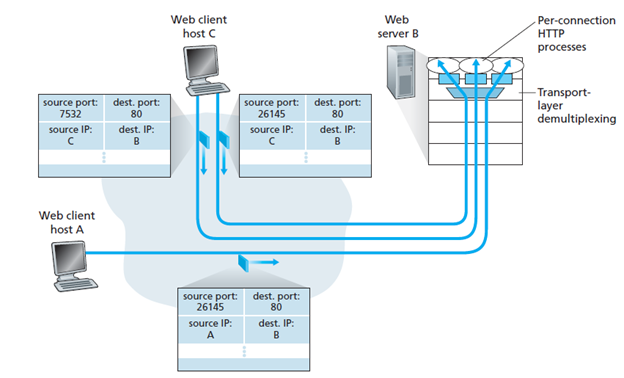
\includegraphics[scale=0.8]{cn1.png}
    \caption{TCP Multiplexing and Demultiplexing}
    \label{fig:my_label}
\end{figure}
\section{User Datagram Protocol (UDP)}
\begin{itemize}
    \item UDP is a connectionless transport layer protocol. It features basic capabilities of transport layer multiplexing/demultiplexing, and basic error checking using checksums.
    
    \item UDP is called connectionless as there is no handshaking between client and server before exchange of data between the two, like there is TCP. 
    
    \item The advantages of UDP are:
    \begin{enumerate}
        \item Smaller packet sizes (8 bytes for UDP header vs 20 bytes for TCP header)
        
        \item No need to maintain connection state unlike in TCP (receive and buffers, congestion control parameters, sequence/acknowledgement numbers are stored in the endpoints), thus less memory overheads for host machines in UDP than in TCP.
        
        \item No delays associated with connection establishment and handshaking
        
        \item Finer application level control on data sent and when:
        \begin{enumerate}
            \item TCP can throttle links as part of its congestion control, and it can also retransmit packets until an acknowledgement of receipt is received from the server. 
            
            \item UDP on the other hand simply packages application layer data into segments and passes them on to the network layer. 
            
            \item For real time applications that often require a minimum sending rate, TCP is not suited. UDP is used, and any functionality over the barebones UDP can be implemented in the application layer. 
        \end{enumerate}
    \end{enumerate}
\end{itemize}
\subsection{UDP Segment Structure}
\begin{itemize}
    \item The UDP segment header consists of 4 fields, each 2 bytes long. The fields are the source port number, destination port number, length of the application data and the checksum value
    
    \item The checksum is the error checking mechanism in UDP.
    
    \item The checksum value is calculated at the sender side by dividing the UDP segment into 16 bit words, taking the sum of all the words (overflows are wrapped around) and then taking the 1s complement of the sum. 
    
    \item The computed checksum value is placed in the checksum field of the UDP segment that is sent. At the receiver side, the checksum of the received UDP segment is compared with the value that was sent. If these 2 values are the same then there were no bit-level errors. 
    
    \item Despite some network layer protocols like IP providing their own error checking, UDP provides the checksum facility so that packets can be transmitted across any links (even the ones that do not provide error checking) and to protect against errors occurring inside routers while in buffer storage. 
    
    \item UDP provides error checking but not error recovery mechanisms. The erroneous segment can either be discarded or passed to the application layer above with a warning, depending on the implementation.
\end{itemize}

\section{Principles of Reliable Data Transfer}
\begin{itemize}
    \item In this context, reliability means that there are no corrupted bits (0 to 1 or 1 to 0), no missing bits and that all data is delivered in the order that it was transmitted. 
    
    \item The reliable data transfer protocol has the responsibility of converting what is essentially an unreliable network layer below it, into a reliable channel. TCP integrates this reliable data transfer as an additional service for applications in the layer above. 
    
    \item At the sender side, the RDT protocol involves a function \texttt{rdt\_send()} that passes the data that the receiving application is to receive. The \texttt{udt\_send()} function passes on the data to the network layer below. 
    
    \item At the receiver side, the function \texttt{rdt\_recv()} function is . The \texttt{rdt\_recv()} catches packets that are entering the system from the unreliable channel. The receiver calls the \texttt{deliver\_data()} function when these packets are to be sent to the application layer.
    
\end{itemize}

\begin{figure}[!h]
    \centering
    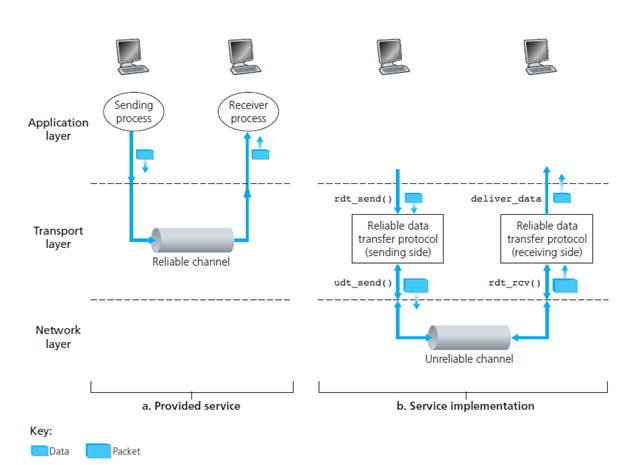
\includegraphics[scale=0.8]{cn2.png}
    \caption{Reliable Data Transfer Protocol}
    \label{fig:my_label_2}
\end{figure}

\subsection{RDT 1.0: Perfectly Reliable Channel}
\begin{itemize}
    \item The first version of RDT protocol assumes that the underlying layers are perfectly reliable and there are no errors possible.
    
    \item The notation for the FSMs shown below is as follows:
    \begin{enumerate}
        \item The states are marked inside the circles
        
        \item The arrows indicate state transition
        
        \item Above the horizontal line is the input at the current state, and below the horizontal line is the action to be taken given the current state and the input. 
    \end{enumerate}
\end{itemize}
\begin{figure}[!ht]
    \centering
    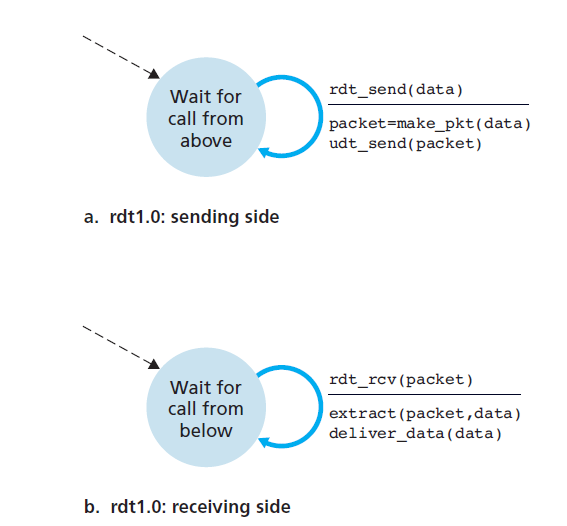
\includegraphics[scale=0.8]{rdt1.png}
    \caption{RDT Version 1.0}
    \label{fig:my_label_3}
\end{figure}
\begin{itemize}
    \item At the sender side, the sender waits for a call for \texttt{rdt\_send(data)} from the application layer. It encapsulates the data in a segment using the \texttt{make\_packet()} function and sends it to the channel using \texttt{udt\_send()}.
    
    \item At the receiver side, the receiver waits for a call for \texttt{rdt\_recv(packet)}. The data is extracted from the packet and it is sent to the application layer above. 
    
    \item It is assumed here that the sender and receiver are sending and receiving at the same rate, so the receiver does not have to ask the sender to slow down the packet rate. 
    
    \item It is also assumed that the channel is perfectly reliable, with no bit-level errors or missing packets possible.
\end{itemize}

\subsection{RDT 2.0: Channel with bit-level errors}
\begin{itemize}
    \item In case a packet has been received at the receiver end with bit level errors (these can be detected using error checking techniques like checksums), the receiver can ask the sender to repeat the packet (ie. send it again).
    
    \item Such protocols where this takes place are called \textbf{Automatic Repeat reQuest} or ARQ protocols. 
    
    \item The extra components of rdt2.0 that make this possible are
    \begin{itemize}
        \item \textbf{Error checking} which requires the sending of additional bits along with the data, that are aggregated in the checksum field of the rdt2.0 segment. 
        
        \item \textbf{Receiver feedback} on whether the packet was delivered properly or with bit level errors. The receiver sends a positive (\textbf{ACK}) or negative (\textbf{NAK}) acknowledgement to this end. 
        
        \item \textbf{Retransmission}, wherein a packet that is received with errors at the receiver side must be sent again by the sender. 
    \end{itemize}
    \item On the sender side, there are two states. In the leftmost state (the start state), the sender waits for the application layer to call \texttt{rdt\_send(data)}. The data is made into a packet called \texttt{sendpkt} (which includes a \textit{checksum}) and sent over the channel using \texttt{udt\_send()}.
    
    \item Once the packet is sent, the sender waits for an ACK/NAK from the receiver side. The acknowledgement is received in the packet called \texttt{recvpkt}. If \texttt{recvpkt} is an ACK (+ve ack), then no action is taken and the sender once again waits for a call from the application layer. 
    
    \item If \texttt{recvpkt} is a NAK (-ve ack), then the sender once again sends the \texttt{sendpkt} packet that it had sent before, and continues to wait for an ACK.
    
    \item At the receiver end, the receiver waits for a packet to arrive from the below layer. 
    
    \item If the packet received (\texttt{recvpkt}) is corrupted, then a NAK packet is created and sent back to the sender.
    
    \item If the \texttt{recvpkt} is not corrupted, the data is extracted and delivered to the app layer above, and an ACK packet is sent back to the sender. 
    
    \item Due to the behaviour of waiting for an ACK and allowing no other communications to take place in the meantime, RDT 2.0 is also called a \textbf{stop and wait} protocol. 
    
    \item The flaw in RDT 2.0 is handling errors that might occur within the ACK and NAK packets themselves, which is handled in RDT 2.1. 
    
    \item Methods of handling corrupt ACK/NAK are:
    \begin{enumerate}
        \item Adding more checksum bits for ACK and NAK
        
        \item Repeating the request every time a garbled ACK/NAK is received. This can cause more delays with every garbled packet that is sent. 
        
        \item Sender resends the packet every time it receives an ACK or NAK. This however introduces duplicate packets into the channel, and the receiver does not know the sequence in which to send ACK/NAK to the packets that it receives. 
    \end{enumerate}
\end{itemize}

\begin{figure}[!h]
    \centering
    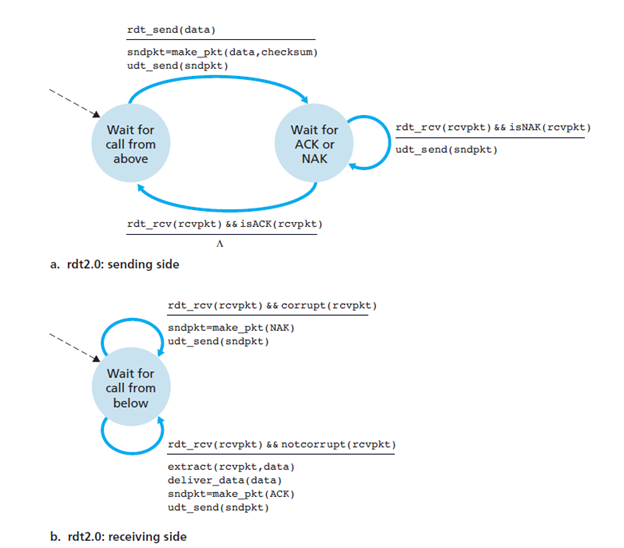
\includegraphics[scale=0.8]{rdt2.png}
    \caption{RDT version 2.0}
    \label{fig:my_label_4}
\end{figure}

\subsection{RDT 2.1: Handling garbled ACKs/NAKs}
\begin{itemize}

    \item RDT 2.1 adds the concept of a \textbf{sequence number} to each packet
    
    \item For a stop and wait protocol, a 1-bit sequence number is sufficient,  since it will allow the receiver to know whether the sender is resending the previously transmitted packet (the sequence number of the received packet has the same sequence number as the most recently received packet) or a new packet (the sequence number moves forward in modulo 2).
    
    \item If the received packet arrives with no errors, an ACK is sent back to the sender. If the received packet has errors, a NAK is sent to the sender. 
\end{itemize}

\begin{figure}[!h]
    \centering
    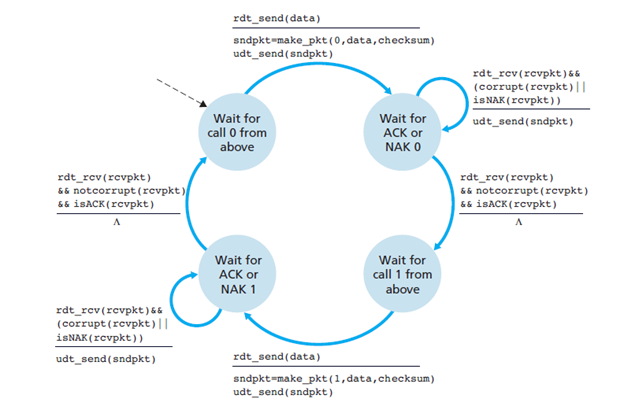
\includegraphics[scale=0.8]{rdt21s.png}
    \caption{RDT version 2.1 Sender}
    \label{fig:my_label_5}
\end{figure}

\begin{figure}[!h]
    \centering
    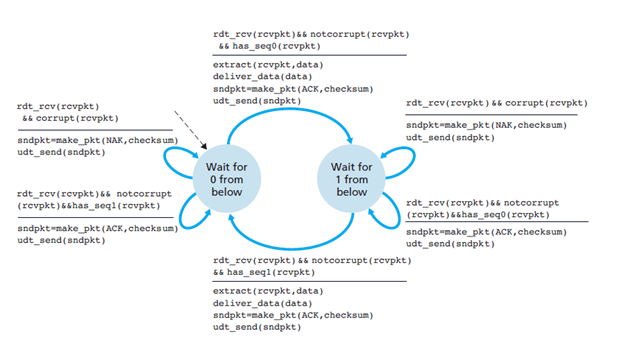
\includegraphics[scale=0.8]{rdt21r.png}
    \caption{RDT version 2.1 Receiver}
    \label{fig:my_label_6}
\end{figure}

\subsection{RDT 2.2: Enhanced version of 2.1}
\begin{itemize}
    \item RDT 2.2 offers the same functionality as RDT 2.1, but without the need for having any NAK packets being sent by the receiver at .
    
    \item  This means that there is no need to implement the \texttt{isNAK()} functions to check packets coming in from the receiver to the sender. 
    
    \item A sender that receives two ACKs for the same packet (that is, receives \textbf{duplicate ACKs}) knows that the receiver did not correctly receive the packet following the packet that is being ACKed twice.
    
    \item The receiver must now include the sequence number of the packet being acknowledged by an ACK message. 
\end{itemize}
\begin{figure}[!h]
    \centering
    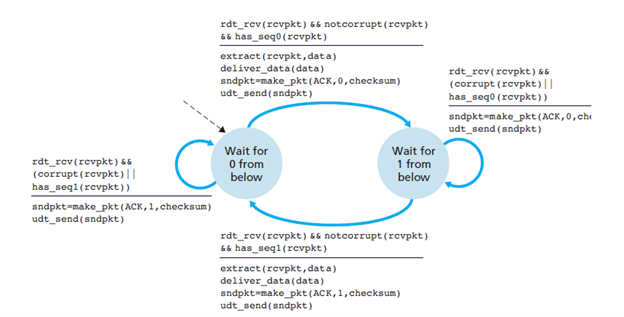
\includegraphics[scale=0.8]{rdt22r.png}
    \caption{RDT version 2.2 Receiver}
    \label{fig:my_label_7}
\end{figure}
\begin{figure}[!h]
    \centering
    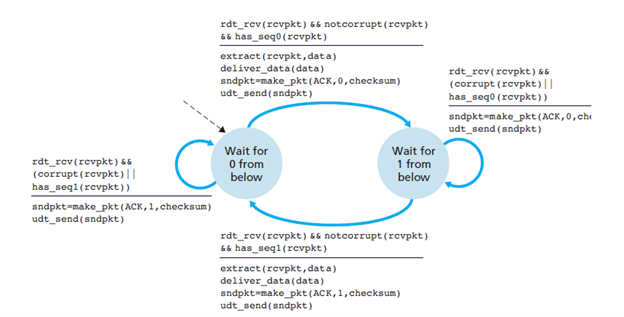
\includegraphics[scale=0.8]{rdt22r.png}
    \caption{RDT version 2.2 Receiver}
    \label{fig:my_label_8}
\end{figure}

\subsection{RDT 3.0: Handling missing packets}
\begin{itemize}
    \item The RDT version 3.0 handles dropped packets using the concept of a \textbf{timer}.
    
    \item The timer represents the \textit{reasonable amount of time} that the sender waits for a positive acknowledgement from the receiver end. The sender is able to start or stop the timer as well as respond to interrupts that the timer generates.
    
    \item In RDT 3.0, retransmission happens if a packet/ACK message is garbled/lost. 
    
    \item If a packet experiences a large delay (but not lost), then the sender will still retransmit as the timer will timeout on the sender side. Hence this leads to duplicate packets in the channel, which is already handled in past versions of RDT (using sequence numbers).  
\end{itemize}

\begin{figure}[!h]
    \centering
    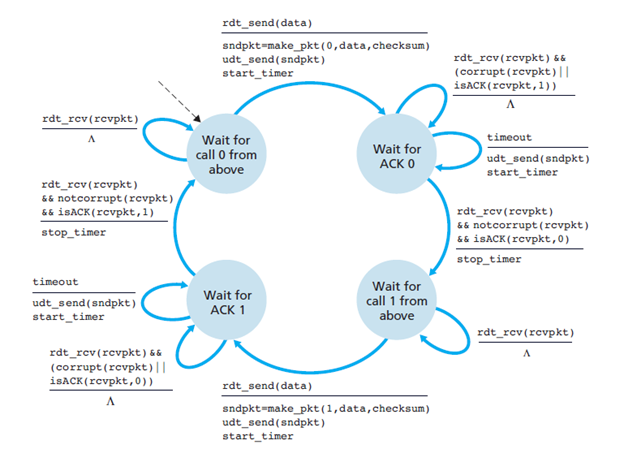
\includegraphics[scale=0.8]{rdt3s.png}
    \caption{RDT version 3.0 Sender}
    \label{fig:my_label_9}
\end{figure}

\begin{figure}[!h]
    \centering
    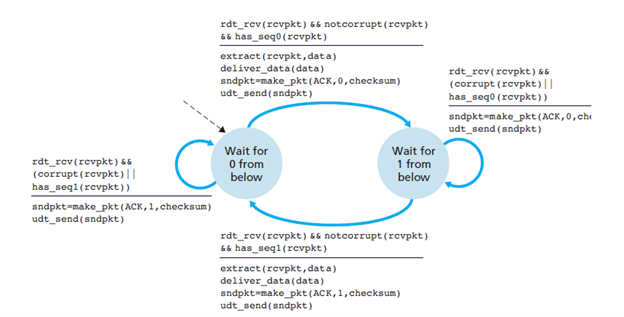
\includegraphics[scale=0.8]{rdt22r.png}
    \caption{RDT version 3.0 Sender}
    \label{fig:my_label_10}
\end{figure}

\section{Pipelined RDT protocols}
\begin{itemize}
    \item In a stop and wait protocol, performance is poor as the sender has to wait for the ACK of the current packet before the next packet can be transmitted. This leads to poor link utilization by the sender.
    
    \item In a pipelined protocol, the sender can send multiple packets at once without having to worry about the receipt of the ACKs for individual packet. 
    
    \item In case one of the packets sent in the pipeline is garbled/lost, retransmission is handled in different methods by different protocols. 
    
    \item Pipelining necessitates the following changes:
    \begin{enumerate}
        \item Increased range for sequence numbers (instead of only 0 and 1), as there are multiple packets in transit at once. 
        
        \item There must be buffers on both sender and receiver sides. The sender will have to buffer packets that have been transmitted but not yet acknowledged. Buffering of correctly received packets may also be needed at the receiver.
    \end{enumerate}
    
    \item The above 2 parameters vary from protocol to protocol. Two common protocols (Go Back N and Selective Repeat) are seen below
\end{itemize}

\subsection{Go Back N (GBN)}
\begin{itemize}
    \item The buffer area on the sender side (also called the \textbf{sliding window}) consists of packets that have \textit{been sent} but \textit{not been ACKed yet}. The size of this window is upto $N$. 
    
    \item If the acknowledgement for a packet is not received within the timeout period, then \textbf{all frames} within the current window are retransmitted. 
    
    \item The sender window size is larger than the receiver window size in a GBN protocol. 
    
    \item Reference: \url{https://youtu.be/QD3oCelHJ20}
\end{itemize}

\subsection{Selective Repeat}
\begin{itemize}

    \item In a selective repeat protocol, only the packets that are dropped/garbled are retransmitted by the sender instead of the entire window at the current time. 
    
    \item The sender window and reciever windows are of the same size in an SR protocol. 
    
    \item SR avoids the performance problems related to GBN flooding the channel with retransmitted packets that might have reached properly but have to be retransmitted because of one dropped packet.
    
    \item Reference: \url{https://youtu.be/WfIhQ3o2xow}
\end{itemize}

\section{Transmission Control Protocol (TCP)}
\begin{itemize}
    \item TCP is a \textbf{connection-oriented}, \textbf{full duplex}, \textbf{point-to-point} transport layer protocol that offers services such as congestion control, flow control and reliable data transfer in addition to the basic transport layer functionalities. 
    
    \item TCP is called connection oriented as a connection must be established between the sender and receiver by means of a \textbf{3-way TCP handshake}.
\end{itemize}
\subsection{TCP 3-Way Handshake}
\begin{itemize}
    \item The steps involved in setting up a TCP connection are:
    \begin{enumerate}
        \item \textbf{SYN}: The client sends a segment to the server with a SYN (with an initial) that informs the server that a connection is to be started, and the starting segment number \texttt{client\_isn} in the sequence number field of the TCP segment. 
        
        \item \textbf{SYN-ACK}: The server allocates the connection variables and buffer space for the connection, and sends a connection-granted response to the client. The acknowledgement number of the header is set to \texttt{client\_isn +1} and the sequence number is \texttt{server\_isn}, which is the initial sequence number for all server-to-client communication. 
        
        \item \textbf{ACK}: In the final part client acknowledges the response of server (by placing the value \texttt{server\_isn+1} in the acknowledgement number field) and they both establish a reliable connection with which they will start the actual data transfer. 
    \end{enumerate}
    \item The SYN and SYN-ACK steps establish the connection parameters for client to server communication (the sequence number), while the SYN-ACK and ACK steps establish conneciton parameters for the server to client direction. 
    
    \item Thus, TCP establishes the full duplex communication. 
    
    \item The largest size of the transport-layer segment is controlled by the \textbf{MSS} (Max Segment Size) parameter. The MSS is determined by checking the length of the largest link-layer frame that can be sent (the \textbf{MTU} or Max Transmission Unit), and then ensuring that the TCP segment + TCP/IP header size will fit in the single link-layer frame. 
\end{itemize}

\subsection{TCP Segment Structure}
\begin{figure}[!h]
    \centering
    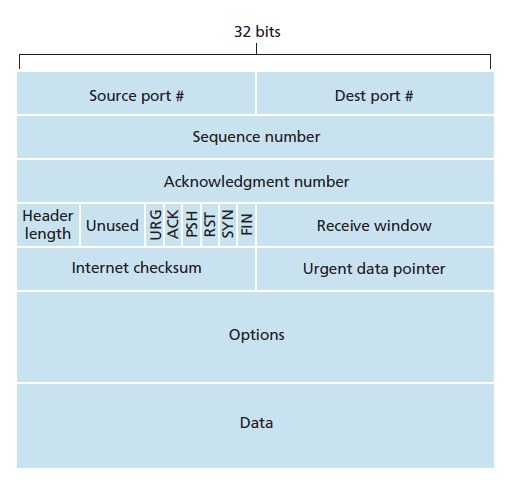
\includegraphics[scale=0.7]{cn3.png}
    \caption{TCP Segment Structure}
    \label{fig:my_label_11}
\end{figure}
\begin{itemize}
    \item 16-bit source and destination port numbers are used for multiplexing and demultiplexing at the end points
    
    \item 32-bit Sequence and Acknowledgement numbers are used to implement RDT. 
    
    \item The 4-bit header length is the length in 32-bit words. 
    
    \item The optional and variable-length options field is used when a sender and receiver negotiate the maximum segment size (MSS) or as a window scaling factor for use in high-speed networks. A time-stamping option is also defined.
    
    \item Theere are 6 flag bits: the \textbf{ACK} bit is set when the ack is sent for a successfully received segment. The \textbf{SYN}, \textbf{FIN} and \textbf{RST} are used for connection set up and teardown. Setting the \textbf{PSH} bit means that the transport layer must pass the data to the application layer immediately, and the \textbf{URG} bit is set when the app layer marks the data as urgent.
    
    \item The 16-bit \textbf{receive window} field is used for flow control. It is used to indicate the number of bytes that a receiver is willing to accept.
    
    \item The \textbf{urgent pointer} is used by TCP to inform the receiving- side upper-layer entity when urgent data exists and pass it a pointer to the end of the urgent data.
\end{itemize}

\subsection{Timeout and RTT Estimation}
\begin{itemize}
    \item Deciding the timeout value when implementing RDT is a complex question. Timeout must be larger than the RTT of the network, but it cannot be too large as that introduces extra latency. 
    
    \item Estimating the actual RTT value is also important. Here, the concept of an \textbf{exponentially weighted moving average} (EWMA) is used. 
    
    \item The \texttt{SampleRTT} for a segment is the interval of time between the sending of the segment (ie. its tranfer to the network layer), and the receipt of the acknowledgement for that segment. 
    
    \item At any point in time, the \texttt{SampleRTT} is measured for only one of the transmitted but unacknowledged segments. Also, \texttt{SampleRTT} is not measured for retransmitted segments, as this could lead to wrong RTT calculations in the case of duplicate acknowledgements. 
    
    \item The estimate of the RTT is calculated as
    \begin{equation}
        EstimatedRTT_{t} = (1-\alpha) EstimatedRTT_{t-1} + \alpha SampleRTT_t
    \end{equation}
    
    The recommmended value for $\alpha$ is 0.125 (RFC 6298). 
    
    \item The deviation in the current \texttt{SampleRTT} from the \texttt{EstimatedRTT} is measured by the quantity \texttt{DevRTT}, which is an EWMA of $|SampleRTT - EstimatedRTT|$
    \begin{equation}
        DevRTT_t = (1-\beta) DevRTT_{t-1} + \beta( |SampleRTT - EstimatedRTT|)
    \end{equation}
    The recommended value for $\beta$ is 0.25 (RFC 6298).
    
    \item The timeout value is calculated from these quantities as
    \begin{equation}
        TimeOut = EstimatedRTT + (4 \times DevRTT)
    \end{equation}
    
    \item An initial timeout value of 1 second is recommended (RFC 6298). When a timeout occurs, the TimeOut value is doubled to ensure that premature timeout does not happen for the next segment. But as soon as the next segment is received then the TimeOut is computed using equation 3 above. 
\end{itemize}

\subsection{TCP Reliable Data Transfer}
\begin{itemize}
    \item In the RDT 3.0 protocol, each transmitted but unacknowledged packet has its own timer associated with it.
    
    \item To avoid timer management overheads, the TCP timer management standard (RFC 6298) specifies a single retransmission timer. 
    
    \item The variable \texttt{sendBase} is the sequence number of the oldest acknowledged byte.
    
    \item Thus \texttt{sendBase}-1 is the sequence number of the last byte that is known to have been received correctly and in order at the receiver.
\end{itemize}

\subsubsection{Doubling timeout interval}
\begin{itemize}
    \item Whenever a timeout event occurs, TCP retransmits the not-yet ACKed segment with the smallest sequence number. At the same time, TCP also doubles the value of the timeout interval. 
    
    \item This action acts like a limited form of congestion control, as timeouts mainly happen due to network congestion, hence instead of retransmitting at a constant rate, TCP retransmits at a longer interval. 
\end{itemize}

\subsubsection{Fast Retransmit}
\begin{itemize}
    \item Whenever a gap occurs in the TCP stream (due to one packet being dropped while sending), the receiver sends duplicate ACKs for the last byte received for all the packets after that gap packet.
    
    \item When the sender receives 3 duplicate acknowledgements for the same data, then it takes this as an indication that the segment following the segment that has been ACKed three times has been lost.
    
    \item In this case, the sender retransmits the missing segment before that segment’s timer expires. This is called a \textbf{fast retransmit}. 
\end{itemize}

\begin{minted}{c}
    int next_seq_num = initial_seq_no;
    int sendBase = initial_seq_no;
    while(true){
        switch(event)
        {
            case Data_recv_from_appLayer:
            {
                Segment = create_new_segment;
                Segment.seqnumber = next_seq_num;
                if(timer not running)
                    start timer;
                pass Segment to Network layer
                next_seq_num = next_seq_num + length(data);
                break;
            }
            case timer_timeout:
            {
                retransmit not-yet-ACKed segment with smallest Seq number;
                start timer;
                break;
            }
            case ACK_recv_with_ACKno_y:
            {
                if(y > sendBase)
                {
                    sendBase = y;
                    if(there are any unACKed segments)
                        start timer;
                    break;
                }else{
                    increment no of dup ACKs received for y
                    if(no_dup_acks_for_y_recvd == 3)
                    {
                        resend segment with seq no=y; /*TCP Fast Retransmit*/
                    }
                }
            }
        } /*End of Switch*/
    } /*End of while loop*/
\end{minted}

\begin{figure}[!ht]
    \centering
    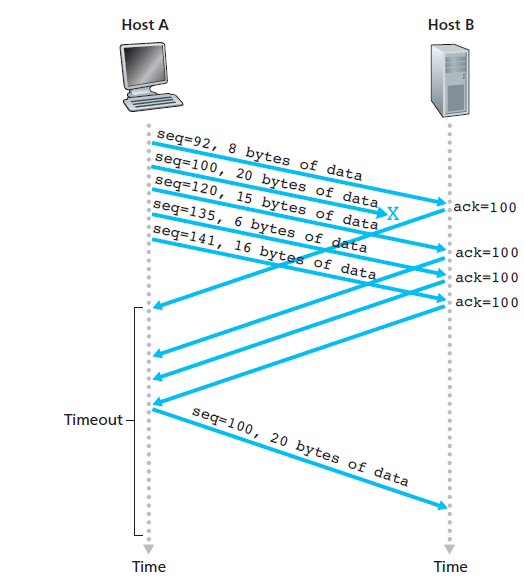
\includegraphics[scale=0.7]{cn4.png}
    \caption{Fast Retransmit in TCP}
    \label{fig:my_label_x}
\end{figure}

\subsection{TCP Flow Control}
\begin{itemize}
    \item The TCP sender maintains a state variable called the \textbf{receiver window}. Informally, this variable defines how much free buffer space is available at the receiver side. 
    
    \item In the receiver, the process keeps track of the number of the last byte read, and the number of the last byte received in the buffer. If the buffer size on the receiver size is $recv\_buffer$  then we must have
    \begin{equation*}
        last\_byte\_recvd- last\_byte\_read \le recv\_buffer
    \end{equation*}
    
    \item The receiver window size \texttt{rwnd} is calculated as 
    \begin{equation*}
        r\_Wnd = recv\_buffer - [last\_byte\_recvd- last\_byte\_read]
    \end{equation*}
    
    \item The sender also keeps track of the numbers of the last byte acked and the last byte sent into the connection. To maintain flow control on the TCP connection, the sender maintains
    \begin{equation*}
        last\_byte\_sent - last\_byte\_acked \le recv\_wnd
    \end{equation*}
    
    \item Consider the case that between hosts A and B, the recv buffer of B becomes full and advertises this to A. So A does not send any packet to B. Once free space appears in B buffer, but B does not have any packets to send to A, hence A is unaware of the newly freed space in B. 
    
    \item In this case above, A is required by the TCP Specification to keep sending 1 byte data to B, and eventually an ACK packet is received by A which indicates that B has non-zero buffer space. 
\end{itemize}

\begin{figure}[!ht]
    \centering
    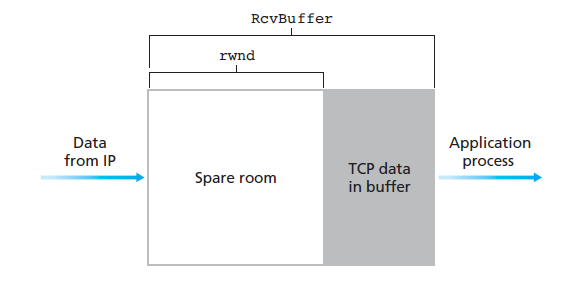
\includegraphics{cn5.png}
    \caption{Receiver side Buffer}
\end{figure}

\begin{figure}[!ht]
    \centering
    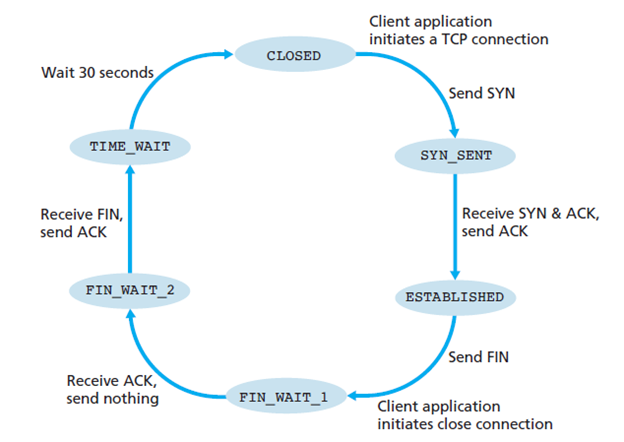
\includegraphics[scale=0.5]{cn6.png}
    \caption{Client TCP States}
\end{figure}

\begin{figure}[!ht]
    \centering
    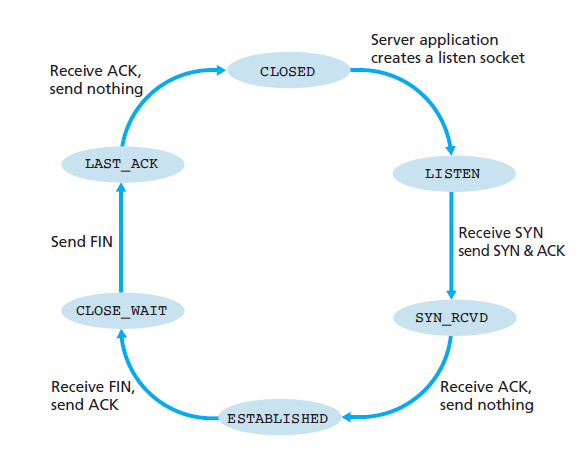
\includegraphics[scale=0.5]{cn7.png}
    \caption{Server TCP States}
\end{figure}

\break

\section{Congestion Control}
\subsection{Costs of congestion in network}
\begin{itemize}
    \item Queueing delays become large as the arrival rate into a router approaches the link rate.
    
    \item The sender must perform retransmissions in order to compensate for dropped (lost) packets due to buffer overflow.
    
    \item Unneeded retransmissions by the sender in the face of large delays (leading to timeout) may cause a router to use its link bandwidth to forward unneeded copies of a packet.
    
    \item When a packet is dropped along a path, the transmission capacity that was used at each of the upstream links to forward that packet to the point at which it is dropped ends up having been wasted. 
\end{itemize}

\subsection{Approaches to Congestion Control}
\begin{itemize}
    \item \textbf{End-to-end}: 
    \begin{itemize}
        \item The transport layer takes full responsibility of congestion control, and the network layer provides no feedback regarding the same.
        
        \item The transport layer infers from events (like dropping of packets) that congestion is present in the network. 
        
        \item This is the approach primarily taken by TCP. TCP uses timeout or triple duplicate ACKs as a signal of congestion. 
    \end{itemize}
    
    \item \textbf{Network-assisted}:
    \begin{itemize}
        \item Network-layer components (routers) provide explicit feedback to the sender regarding the congestion state in the network.
        
        \item Simplest approaches indicate one single hardware bit indicating N/w congestion or not, or the sending of a \textbf{choke packet} from the router to the sender indicating congestion. 
        
        \item More complex mechanisms for congestion control like ATM ABR allow a router to inform the sender explicitly of the transmission rate it (the router) can support on an outgoing link.
    \end{itemize}
\end{itemize}

\subsection{TCP Congestion Control}
\begin{itemize}
    \item The sender maintains an additional TCP variable to enforce congestion control, called the \textbf{congestion window} (\texttt{cwnd}). The cwnd value is a constraint on the aount of data that can be sent. We must always have:
    \begin{equation*}
        last\_byte\_sent - last\_byte\_acked \le min(recv\_wnd, cwnd)
    \end{equation*}
    
    \item The sender rate can be roughly calculated as $\frac{cwnd}{RTT}$, as at the beginning of an RTT, the sender can send cwnd bytes of information. Increasing \texttt{cwnd} increases sender rate. 
    
    \item A \textit{loss event} is defined as either a \textbf{timeout} or the receipt of \textbf{triple duplicate ACKs} (the fast retransmit case). 
    
    \item The value of \texttt{cwnd} is decided by the following general guidelines:
    \begin{itemize}
        \item Lost segment implies connection, hence \texttt{cwnd} should reduce. 
        
        \item ACK received by sender implies no congestion, hence hence \texttt{cwnd} can be increased.
        
        \item \textit{Bandwidth probing}: The practice of slowly increasing the sender rate until the point that congestion occurs, then slowly reducing from that point. After backing off, the sender once again probes to see if the network's congestion has changed or not. 
    \end{itemize}
\end{itemize}

\subsubsection{Slow Start}
\begin{itemize}
    \item The inital value of \texttt{cwnd} is set to $1\times MSS$. Every time a transmitted segment is acknowledged, the \texttt{cwnd} increases by 1 MSS. 
    
    \item First one MSS is sent, once it is ACKed, the cwnd becomes 2MSS and 2 MSS packets are sent out. For each positive ACK, the cwnd increases by one MSS, hence from 2MSS the cwnd becomes 4MSS. 
    
    \item Hence, in every RTT, the \texttt{cwnd} becomes double (exponential growth). 
    
    \item If a timeout occurs, the cwnd is set to 1 MSS and slow start process is repeated again. At the first timeout, the \texttt{ssthresh} (slow start threshold) is set to \texttt{cwnd/2} (half of the value of cwnd at which the loss event occurred). 
    
    \item Subsequently, if \texttt{cwnd} exceeds \texttt{ssthresh} then TCP transitions to the \textit{congestion avoidance} state.
    
    \item If 3 duplicate ACKs are received, then TCP performs a fast retransmit and enters the \textit{fast recovery} state.
\end{itemize}

\subsubsection{Congestion Avoidance}
\begin{itemize}
    \item  In this state, the cwnd value increases linearly rather than exponentially over a single RTT. 
    
    \item When a timeout occurs in congestion avoidance mode, the \texttt{ssthresh} is set to \texttt{cwnd/2}, and the \texttt{cwnd} is updated to 1 MSS. 
    
    \item When 3 duplicate ACKs are received in congestion avoidance mode, TCP enters the fast recovery mode. The \texttt{ssthresh} is set to half the cwnd value when 3 dup ACKs were received, and then the cwnd is updated to half that value with 3 MSS added ($cwnd = cwnd/2 + 3MSS$. 
\end{itemize}

\subsubsection{Fast Recovery}
\begin{itemize}
    \item This is an optional component of TCP congestion control mechanism. 
    
    \item In fast recovery state, the cwnd is increased by 1 MSS for every duplicate ACK received. When the missing ACK arrives, the cwnd is set back to ssthresh, and it enters congestion avoidance mode. 
    
    \item In the fast recovery state, if a timeout event occurs, the ssthresh is set to cwnd/2 cwnd size is set to 1, and TCP enters Slow Start. 
    
    \item In the recent version of TCP (called \textbf{TCP Reno}) fast recovery is used. 
    
    \item In the older version \textbf{TCP Tahoe}, the ssthresh is set to cwnd/2 and cwnd is cut to 1 MSS irrespective of what loss event happened. 
\end{itemize}

\begin{figure}
    \centering
    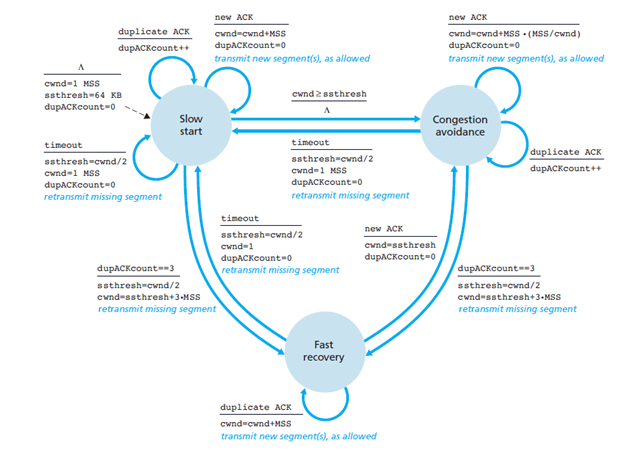
\includegraphics[scale=0.9]{cn8.png}
    \caption{TCP Congestion Control}
    \label{fig:my_label_15}
\end{figure}
\end{document}